%%%%%%%%%%%%%%%%%%%%%%%%%%%%%%%%%%%%%%%%
% Structured General Purpose Assignment
% LaTeX Template
%
% This template has been downloaded from:
% http://www.latextemplates.com
%
% Original author:
% Ted Pavlic (http://www.tedpavlic.com)
%
% Note:
% The \lipsum[#] commands throughout this template generate dummy text
% to fill the template out. These commands should all be removed when 
% writing assignment content.
%
%%%%%%%%%%%%%%%%%%%%%%%%%%%%%%%%%%%%%%%%%

%----------------------------------------------------------------------------------------
%       PACKAGES AND OTHER DOCUMENT CONFIGURATIONS
%----------------------------------------------------------------------------------------

\documentclass{article}

\usepackage{fancyhdr} % Required for custom headers
\usepackage{lastpage} % Required to determine the last page for the footer
\usepackage{extramarks} % Required for headers and footers
\usepackage{graphicx} % Required to insert images
\usepackage{lipsum} % Used for inserting dummy 'Lorem ipsum' text into the template
\usepackage{subcaption}
\usepackage{algorithm}
\usepackage{algpseudocode}
\usepackage{pifont}


\usepackage{amsmath}

% Margins
\topmargin=-0.45in
\evensidemargin=0in
\oddsidemargin=0in
\textwidth=6.5in
\textheight=9.0in
\headsep=0.25in 

\linespread{1.1} % Line spacing

% Set up the header and footer
\pagestyle{fancy}
\lhead{\hmwkAuthorName} % Top left header
\chead{\hmwkClass\ : \hmwkTitle} % Top center header
\rhead{\firstxmark} % Top right header
\lfoot{\lastxmark} % Bottom left footer
\cfoot{} % Bottom center footer
\rfoot{Page\ \thepage\ of\ \pageref{LastPage}} % Bottom right footer
\renewcommand\headrulewidth{0.4pt} % Size of the header rule
\renewcommand\footrulewidth{0.4pt} % Size of the footer rule

\setlength\parindent{0pt} % Removes all indentation from paragraphs

%----------------------------------------------------------------------------------------
%       DOCUMENT STRUCTURE COMMANDS
%       Skip this unless you know what you're doing
%----------------------------------------------------------------------------------------

% Header and footer for when a page split occurs within a problem environment
\newcommand{\enterProblemHeader}[1]{
\nobreak\extramarks{#1}{#1 continued on next page\ldots}\nobreak
\nobreak\extramarks{#1 (continued)}{#1 continued on next page\ldots}\nobreak
}

% Header and footer for when a page split occurs between problem environments
\newcommand{\exitProblemHeader}[1]{
\nobreak\extramarks{#1 (continued)}{#1 continued on next page\ldots}\nobreak
\nobreak\extramarks{#1}{}\nobreak
}

\setcounter{secnumdepth}{0} % Removes default section numbers
\newcounter{homeworkProblemCounter} % Creates a counter to keep track of the number of problems

\newcommand{\homeworkProblemName}{}
\newenvironment{homeworkProblem}[1][Problem \arabic{homeworkProblemCounter}]{ % Makes a new environment called homeworkProblem which takes 1 argument (custom name) but the default is "Problem #"
\stepcounter{homeworkProblemCounter} % Increase counter for number of problems
\renewcommand{\homeworkProblemName}{#1} % Assign \homeworkProblemName the name of the problem
\section{\homeworkProblemName} % Make a section in the document with the custom problem count
\enterProblemHeader{\homeworkProblemName} % Header and footer within the environment
}{
\exitProblemHeader{\homeworkProblemName} % Header and footer after the environment
}

\newcommand{\problemAnswer}[1]{ % Defines the problem answer command with the content as the only argument
\noindent\framebox[\columnwidth][c]{\begin{minipage}{0.98\columnwidth}#1\end{minipage}} % Makes the box around the problem answer and puts the content inside
}

\newcommand{\homeworkSectionName}{}
\newenvironment{homeworkSection}[1]{ % New environment for sections within homework problems, takes 1 argument - the name of the section
\renewcommand{\homeworkSectionName}{#1} % Assign \homeworkSectionName to the name of the section from the environment argument
\subsection{\homeworkSectionName} % Make a subsection with the custom name of the subsection
\enterProblemHeader{\homeworkProblemName\ [\homeworkSectionName]} % Header and footer within the environment
}{
\enterProblemHeader{\homeworkProblemName} % Header and footer after the environment
}
   
%----------------------------------------------------------------------------------------
%       NAME AND CLASS SECTION
%----------------------------------------------------------------------------------------

\newcommand{\hmwkTitle}{Assignment\ \#5 } % Assignment title
\newcommand{\hmwkDueDate}{Tueday,\ November\ 17,\ 2015(One late day used)} % Due date
\newcommand{\hmwkClass}{CSCI-567} % Course/class
\newcommand{\hmwkClassTime}{} % Class/lecture time
\newcommand{\hmwkAuthorName}{Saket Choudhary} % Your name
\newcommand{\hmwkAuthorID}{2170058637} % Teacher/lecturer
%----------------------------------------------------------------------------------------
%       TITLE PAGE
%----------------------------------------------------------------------------------------

\title{
\vspace{2in}
\textmd{\textbf{\hmwkClass:\ \hmwkTitle}}\\
\normalsize\vspace{0.1in}\small{Due\ on\ \hmwkDueDate}\\
\vspace{0.1in}\large{\textit{\hmwkClassTime}}
\vspace{3in}
}

\author{\textbf{\hmwkAuthorName} \\
        \textbf{\hmwkAuthorID}
        }
\date{} % Insert date here if you want it to appear below your name

%----------------------------------------------------------------------------------------

\begin{document}

\maketitle

%----------------------------------------------------------------------------------------
%       TABLE OF CONTENTS
%----------------------------------------------------------------------------------------

%\setcounter{tocdepth}{1} % Uncomment this line if you don't want subsections listed in the ToC

\newpage
\tableofcontents
\newpage








\begin{homeworkProblem}[Problem 1] % Custom section title
\begin{homeworkSection}{\homeworkProblemName: ~(a)}

\problemAnswer{
	To find $\nabla_{y_t} L$:
	
	\begin{align*}
	\nabla_{y_t}L &= \frac{\partial}{\partial y_t} \frac{1}{2}\sum_{i=1}^{N}(y_i-\hat{y_i})^T(y_i-\hat{y_i})\\
	&=  \frac{\partial}{\partial y_t} \frac{1}{2} \sum_{i=1}^{N}(y_i^Ty_i-2y_i^T\hat{y_i}+\hat{y_t}^2)\\
	&= \frac{1}{2} (2y_t-2\hat{y_t})\\
	&= y_t-\hat{y_t}
	\end{align*}
	
	$$
		\boxed{\nabla_{y_t}L  =  y_t-\hat{y_t}}
	$$
	
}
		\end{homeworkSection}
		
	\begin{homeworkSection}{\homeworkProblemName: ~(b)}
	\problemAnswer{
		To find $\nabla_{y_t} L$:
		
		\begin{align*}
		\nabla_{s_t}L &= \sum_{k=1}^T \frac{\partial L}{\partial y_k} \times \frac{\partial y_k}{\partial s_k} \times \frac{\partial s_k}{\partial s_t}
		\end{align*}
		
	
		
	
		
		Let's define $z_t = W_{IH}x_t+W_{HH}s_{t-1}$
		
		Thus,
		\begin{align*}
		z_k &= W_{IH}x_k+W_{HH}s_{k-1}\\
		s_k &= \sigma(z_k)\\
		y_k &= W_{HO}s_k
		\end{align*}
		
		Thus,
		\begin{align}
		\frac{\partial y_k}{\partial s_k} &= W_{HO}\\
		\frac{\partial s_k}{\partial z_k} &= \sigma(z_k)(1-\sigma(z_k))\\
		\frac{\partial z_k}{\partial W_{IH}} &= x_k\\
		\frac{\partial y_k}{\partial W_{HH}} &= y_{k-1}\\
		\frac{\partial z_k}{\partial s_{k-1}} &= W_{HH}\\
		 \frac{\partial s_k}{\partial s_{k-1}} &= \frac{\partial s_k}{\partial z_k} \frac{\partial z_k}{\partial s_{k-1}} = \sigma(z_k)(1-\sigma(z_k))W_{HH}
		\end{align}
		
		 	Let's now consider $ \frac{\partial s_k}{\partial s_t}$:
		 	
		 	$s_k$ depends on $s_{k-1},s_{k-2},\dots s_{1}$.
		 	And hence:
		 	
		 	\begin{align*}
		 	\frac{\partial s_k}{\partial s_t} &= 0\ \forall\ k<t 
		 	\end{align*}
		 	
		 For $k\geq t$:
		 
		\begin{align*}
		\frac{\partial s_k}{\partial s_t} &= \frac{\partial s_k}{\partial s_{k-1}} \times \frac{\partial s_{k-1}}{\partial s_{k-2}} \times \frac{\partial s_{k-2}}{\partial s_{k-3}} \times \dots \frac{\partial s_{k-(k-t)+1}}{\partial s_{k-(k-t)}} 
		\end{align*} 
		
		
		
		Thus, consider a special case of $t=T$:
		
		\begin{align*}
		\nabla_{s_T}L &= \sum_{k=T}^T \frac{\partial L}{\partial y_k} \times \frac{\partial y_k}{\partial s_k} \times \frac{\partial s_k}{\partial s_t}\\
		&= \frac{\partial L}{\partial y_T} \times \frac{\partial y_T}{\partial s_T}\\
		&= (y_T-\hat{y_T})W_{HO}
		\end{align*}
		
		
		Thus,
		$$
		\boxed{\nabla_{S_T} L = (y_T-\hat{y_T})W_{HO}}
		$$
	}
	\problemAnswer{
		Let's consider $\nabla_{s_{t}}L$ and $\nabla_{s_{t+1}}L$:
		
		\begin{eqnarray*}
		\nabla_{s_{t+1}}L =  \sum_{k=t+1}^T \frac{\partial L}{\partial y_k} \times \frac{\partial y_k}{\partial s_k} \times \frac{\partial s_k}{\partial s_t}\\
		\nabla_{s_{t}}L =  \sum_{k=t}^T \frac{\partial L}{\partial y_k} \times \frac{\partial y_k}{\partial s_k} \times \frac{\partial s_k}{\partial s_t}\\
		\implies \nabla_{s_{t}}L = \nabla_{s_{t+1}}L +   \frac{\partial L}{\partial y_t} \times \frac{\partial y_t}{\partial s_t} \times \frac{\partial s_t}{\partial s_t}\\
		\implies \nabla_{s_{t}}L = \nabla_{s_{t+1}}L + (y_t-\hat{y_t})W_{HO}
		\end{eqnarray*}	
		
		
		Thus,
		$$
		\boxed{\nabla_{s_{t}}L = \nabla_{s_{t+1}}L + (y_y-\hat{y_t})W_{HO}}
		$$
		
		
	}
\end{homeworkSection}

\begin{homeworkSection}{\homeworkProblemName: ~(c)}
	\problemAnswer{
		
		\begin{align*}
		\nabla_{W_{IH}}L &= \sum_{k=1}^T \big(\frac{\partial L}{\partial y_k} \times \frac{\partial y_k}{\partial s_k}\big) \times \frac{\partial s_k}{ \partial z_k} \times \frac{\partial z_k}{\partial W_{IH}}\\
		&= \sum_{k=1}^T (y_k-\hat{y_k})W_{HO} \times \sigma(z_k)(1-\sigma(z_k)) \times x_k 
		\end{align*}
		
		Thus,\\
		\problemAnswer{
		\begin{eqnarray*}
			\nabla_{W_{IH}}L = \sum_{k=1}^(y_k-\hat{y_k})W_{HO} \times \sigma(z_k)(1-\sigma(z_k)) \times x_k\\
			\text{where } \nabla_{s_{k}}L = \nabla_{s_{k+1}}L + (y_k-\hat{y_k})W_{HO}\\
			\text{and } z_k = W_{IH}x_k+W_{HH}s_{k-1}	\\
			\text{boundary condition } \nabla_{S_T}L =  (y_T-\hat{y_T})W_{HO}
		\end{eqnarray*}}
		
			\begin{align*}
			\nabla_{W_{HH}}L &= \sum_{k=1}^T \big(\frac{\partial L}{\partial y_k} \times \frac{\partial y_k}{\partial s_k}\big) \times \frac{\partial s_k}{ \partial z_k} \times \frac{\partial z_k}{\partial W_{HH}}\\
			&= \sum_{k=1}^T (y_k-\hat{y_k})W_{HO} \times \sigma(z_k)(1-\sigma(z_k)) \times s_{k -1}
			\end{align*}
			
		Thus,\\
		\problemAnswer{
			\begin{eqnarray*}
				\nabla_{W_{IH}}L = \sum_{k=1}^T (y_k-\hat{y_k})W_{HO} \times \sigma(z_k)(1-\sigma(z_k)) \times s_{k -1}\\
				\text{where } \nabla_{s_{k}}L = \nabla_{s_{k+1}}L + (y_k-\hat{y_k})W_{HO}\\
				\text{and } z_k = W_{IH}x_k+W_{HH}s_{k-1}	\\
				\text{boundary condition } \nabla_{S_T}L =  (y_T-\hat{y_T})W_{HO}
			\end{eqnarray*}}
	
		}
		\problemAnswer{
			
			
			\begin{align*}
			\nabla_{W_{HO}}L &= \sum_{k=1}^T \frac{\partial L}{\partial y_k} \times \frac{\partial y_k}{\partial W_{HO}}\\
			&= \sum_{k=1}^T (y_k-\hat{y_k})s_k
			\end{align*}
			
			Thus,
			
			\problemAnswer{
				\begin{eqnarray*}
					\nabla_{W_{HO}}L =\sum_{k=1}^T (y_k-\hat{y_k})s_k
				\end{eqnarray*}
				
				
			
			}
			
			}
\end{homeworkSection}	

\begin{homeworkSection}{\homeworkProblemName: ~(d)}
	\problemAnswer{
		Leaky hidden units:
		$$
		s_t = (1-\tau)s_{t-1} + \tau \sigma(z_t) 
		$$
		
		Thus,
		\begin{align*}
		\frac{\partial s_t}{\partial s_{t-1}} &= 1-\tau + \tau \sigma(z_t)(1-\sigma(z_t))W_{HH}\\
		\frac{\partial s_t}{\partial z_t} &= \tau \sigma(z_t)(1-\sigma(z_t))
		\end{align*}
			
			For $\nabla_{W_{IH}}L$,
			\begin{align*}
			\nabla_{W_{IH}}L &= \sum_{k=1}^T \big(\frac{\partial L}{\partial y_k} \times \frac{\partial y_k}{\partial s_k}\big) \times \frac{\partial s_k}{ \partial z_k} \times \frac{\partial z_k}{\partial W_{IH}}\\
			&= \sum_{k=1}^T (y_k-\hat{y_k})W_{HO} \times \tau \sigma(z_k)(1-\sigma(z_k)) \times x_k 
			\end{align*}
			
			For $\nabla_{W_{HH}}L$,
			\begin{align*}
			\nabla_{W_{IH}}L &= \sum_{k=1}^T \big(\frac{\partial L}{\partial y_k} \times \frac{\partial y_k}{\partial s_k}\big) \times \frac{\partial s_k}{ \partial z_k} \times \frac{\partial z_k}{\partial W_{HH}}\\
			&= \sum_{k=1}^T (y_k-\hat{y_k})W_{HO} \times \tau \sigma(z_k)(1-\sigma(z_k)) \times s_{k-1} 
			\end{align*}
			
			For $\nabla_{W_{HO}}L$,
			\begin{align*}
			\nabla_{W_{HO}}L &= \sum_{k=1}^T (y_k-\hat{y_k})s_k\\
			&=  \sum_{k=1}^T (y_k-\hat{y_k})((1-\tau)s_{k-1}+\tau\sigma(z_k))
			\end{align*}

		}
\end{homeworkSection}

\end{homeworkProblem}

\begin{homeworkProblem}[Problem 2]
	\begin{homeworkSection} {\homeworkProblemName: ~(a)}
		\problemAnswer{
			$$
			\tilde{D} = \sum_{n=1}^N\sum_{k=1}^K r_{nk} ||\phi(x_n) - \tilde{\mu_k}||^2
			$$
			where $$
			\tilde{\mu_k} = \frac{\sum_{i=1}^N r_{ik}\phi(x_i)}{\sum_{i=1}^N r_{ik}}
			$$
			Consider, $||\phi(x_n) - \tilde{\mu_k}||^2$
			\begin{align*}
			||\phi(x_n) - \tilde{\mu_k}||^2 &= (\phi(x_n)- \tilde{\mu_k})^T(\phi(x_n)-\tilde{\mu_k})\\
			&=\phi(x_n)^T\phi(x_n) - 2\tilde{\mu}^T\phi(x_n) + \tilde{\mu}^T\tilde{\mu}\\
			&= \phi(x_n)^T\phi(x_n) -2 \frac{\sum_{i=1}^N r_{ik}\phi(x_i)^T\phi(x_n)}{\sum_{i=1}^N r_{ik}} + \frac{\sum_{i=1}^N \sum_{j=1}^Nr_{ik}r_{jk}\phi(x_i)^T\phi(x_j)}{\sum_{i=1}^N \sum_{j=1}^N r_{ik}r_{jk}}
			\end{align*}

		Define $n_k = \sum_{i=1}^N r_{ik}$, so that it simplifies to:
		\begin{align*}
		||\phi(x_n) - \tilde{\mu_k}||^2 &= \phi(x_n)^T\phi(x_n) -2 \frac{\sum_{i=1}^N r_{ik}\phi(x_i)^T\phi(x_n)}{n_k} + \frac{\sum_{i=1}^N \sum_{j=1}^Nr_{ik}r_{jk}\phi(x_i)^T\phi(x_j)}{n_k^2}\\
		&= K(x_n,x_n) -2 \frac{\sum_{i=1}^N r_{ik} K(x_i, x_n)}{n_k} + \frac{\sum_{i=1}^N \sum_{j=1}^Nr_{ik}r_{jk}K(x_i,x_j)}{n_k^2}
		\end{align*}
			
			Thus,
			$$
			\tilde{D} = \sum_{n=1}^N K(x_n,x_n) -2 \frac{\sum_{i=1}^N r_{ik} K(x_i, x_n)}{n_k} + \frac{\sum_{i=1}^N \sum_{j=1}^Nr_{ik}r_{jk}K(x_i,x_j)}{n_k^2}
			$$
			}		
	\end{homeworkSection}

\begin{homeworkSection}{\homeworkProblemName: ~(b)}
	\problemAnswer{
		\begin{enumerate}
			\item For given point $x_n$ calculate $K(x_n,x_n) -2 \frac{\sum_{i=1}^N r_{ik} K(x_i, x_n)}{n_k} + \frac{\sum_{i=1}^N \sum_{j=1}^Nr_{ik}r_{jk}K(x_i,x_j)}{n_k^2}$ for all possible clusters $k$
			\item Assign cluster to point $x_n$ using:
			$$
			r_{nk} = \begin{cases}
			1 & k = \arg \min_k ||\phi(x_n)-\tilde{u_k}||_2^2\\
			0 & \text{otherwise}
			\end{cases}
			$$
			
			where 
			$$
			K(x_n,x_n) -2 \frac{\sum_{i=1}^N r_{ik} K(x_i, x_n)}{n_k} + \frac{\sum_{i=1}^N \sum_{j=1}^Nr_{ik}r_{jk}K(x_i,x_j)}{n_k^2}
			$$ and $n_k = \sum_{i=1}^N r_{ik}$
			
			
		\end{enumerate}
		}
\end{homeworkSection}
\clearpage

\begin{homeworkSection}{\homeworkProblemName: ~(c)}
%\problemAnswer{
	\begin{algorithm}
		\caption{Kernel k means}
		\begin{algorithmic}[1]
		\Procedure{Kernel K means} {}
		\State mu[i] = x(random(1..N)) for $1 \leq i \leq k$ 		\Comment initialise cluster centroids[1..k]  randomly choosing any $k$ points of $N$ (Sample without replacement)
		\For i:1 to N
			\For j:1 to N
				K[i,j] = $\phi(x_i)\phi(x_j)$
			\EndFor 
		\EndFor 

		
		r(n,k) $\longleftarrow$ $[0]$
		\For i:1 to N


		\State	j = $\arg \min_k ||\phi(x_n)-\mu_k||^2$		\Comment Use the above formula to calculate distances
		\State	r[i,j] = 1
		\State Update $mu_j$ 		\Comment Recalculate centroids of assigned cluster $j$
		\EndFor
		
				\EndProcedure
		\end{algorithmic}
		
	\end{algorithm}
%	}
\end{homeworkSection}

\end{homeworkProblem}

\begin{homeworkProblem}[Problem 3]
	\problemAnswer{
		Given:
		$$
		p(x_i) = \begin{cases}
		\pi+(1-\pi)e^{-\lambda} & x_i=0\\
		(1-\pi)\frac{\lambda^{x_i}e^{-\lambda}}{x_i!} & x_i>0
		\end{cases}
		$$
		
		Alternatively:
		
		$$
		X_i = \begin{cases}
		0 & \text{probability = }  \pi+(1-\pi)e^{-\lambda}\\
		x_i & \text{probability = } (1-\pi)\frac{\lambda^{x_i}e^{-\lambda}}{x_i!}
		\end{cases}
		$$
		
		We define a $latent$ variable $Z_i$ for all cases where $X_i=0$. It is latent because when we observed $X_i=0$ we do not know if it came out of the 'Poisson' distribution or it came out the 'degenerate' distribution(which has a probability of $1$ at point 0.).  we cannot observe the following. So $X_i$ comes out of a mixture of a degenerate distribution as follows:
		
		$$
		Z_i = \begin{cases}
		1 &  \text{$X_i$ is from the degenerate distrbution }\\
		0 & \text{otherwise}
		\end{cases}
		$$
		
		\begin{eqnarray*}
		p(X_i=0,Z_i=1) = p(Z_i=1) \times p(X_i=0|Z_i=1) = \pi \times 1\\
		P(X_i=0,Z_i=0) = p(Z_i=0) \times p(X_i=0|Z_i=0) = (1-\pi)e^{-\lambda} \times 1
		\end{eqnarray*}
		
		\begin{align*}
		L((\pi,\lambda)|(X,Z)) &= \prod_{x_i=0} \pi^{z_i} \times ((1-\pi)e^{-\lambda})^{1-z_i} \times \prod_{x_i > 0} (1-\pi)e^\frac{\lambda^x_i e^{-\lambda}}{x_i!}\\
		\log L &= \sum_{I(x_i=0)} z_i \log(\pi) + (1-z_i) \big( \log(1-\pi) - \lambda \big)\\  &+ \sum_{I(x_i>0)} \big( \log(1-\pi) + x_i \log(\lambda_i) - \lambda - \log(x_i!) \big)
		\end{align*}
		
		Notation $\theta = (\pi, \lambda)$ $\theta_0$ represents a known parameter(as estimated from previous step, I don't use explicit indices for showing the E,M steps)
	}
	\problemAnswer{
\textbf{		E step:}
		
\begin{align*}	
		Q(\theta, \theta_0) &= \sum_{I(x_i=0)} E_{P(Z|X)}[z_i] \log(\pi) + (1-E_{P(Z|X)}[z_i]) \big( \log(1-\pi) - \lambda \big)\\  
		&+ \sum_{I(x_i>0)} \big( \log(1-\pi) + x_i \log(\lambda_i) - \lambda - \log(x_i!) \big)
\end{align*}

\begin{align*}	
E_{P(Z|X_i)}[z_i] &= 0 \times p(Z_i=0|X) + 1 \times p(Z_i=1|X_i=0) \\
&= \frac{p(X_i=0|Z_i=1)p(Z_i=1)}{p(X_i=0|Z_i=0)p(Z_i=0)+p(X_i=0|Z_i=1)p(Z_i=1)}\\
&= \frac{\pi_0}{\pi_0+(1-\pi_0)e^{-\lambda_0}}
\end{align*}

Hence,
\begin{align*}
Q(\theta, \theta_0) &= \sum_{I(x_i=0)} \frac{\pi_0}{\pi_0+(1-\pi_0)e^{-\lambda_0}} \log(\pi) + (\frac{(1-\pi_0)e^{-\lambda_0}}{\pi_0+(1-\pi_0)e^{-\lambda_0}}) \big( \log(1-\pi) - \lambda \big)\\  
&+ \sum_{I(x_i>0)} \big( \log(1-\pi) + x_i \log(\lambda) - \lambda - \log(x_i!) \big)
\end{align*}

\textbf{M step:}
\begin{align*}
\frac{\partial Q}{\partial \lambda} &=0\\
&= \sum_{I(x_i=0)} (1-E[z_i])(-1) + \sum_{I(x_i>0)} (\frac{x_i}{\lambda}-1)  =0\\
\implies \hat{\lambda} &= \frac{\sum_{I(x_i>0)}x_i}{n-\sum_{I(x_i=0)}E[z_i]} \\
\hat{\lambda}  &= \frac{\sum_{I(x_i>0)}x_i}{n-\sum_{I(x_i=0)}\hat{z_i}} \\
\text{where } \hat{z} &= \frac{\pi_0}{\pi_0+(1-\pi_0)e^{-\lambda_0}}
\end{align*}
		

\begin{align*}
\frac{\partial Q}{\partial \pi} &=0\\
&=  \sum_{I(x_i=0)} \big(\frac{E[z_i]}{\pi} - \frac{1-E[z_i]}{1-\pi}\big) - \sum_{I(x_i>0)}  \frac{1}{1-\pi} =0 \\
&= \sum_{I(x_i=0)} \big(\frac{E[z_i]}{\pi} + \frac{E[z_i]}{1-\pi}\big) - \frac{n}{1-\pi} = 0\\
\implies \hat{\pi} &= \sum_{I(x_i=0)} \frac{\hat{z_i}}{n}
\end{align*}
	}
	\problemAnswer{
		Thus parameter updates are as follows:(subscript 1 indicates the next iteration and 0 indicates known parameter value from previous step)
		$$
		\boxed{\hat{z}_1 = \frac{\pi_0}{\pi_0+(1-\pi_0)e^{-\lambda_0}} }
		$$
		
		$$
		\boxed{\hat{\lambda}_1 = \frac{\sum_{I(x_i>0)}x_i}{n-\sum_{I(x_i=0)}\hat{z_1}}}
		$$
		
		$$
		\boxed{ \hat{\pi} = \sum_{I(x_i=0)} \frac{\hat{z_1}}{n} }
		$$
		
		
		}
\end{homeworkProblem}
%\clearpage

\begin{homeworkProblem}[Problem 4]
\begin{homeworkSection}{Problem 4.2}
	\problemAnswer{As seen from Figure 2, k-means algorithm fails to separate the two circles. This happens because of the failure of the following assumption in this case: the dataset is linearly separable. The circular dataset is not really separable, and hence the clusters returned by k-means, have a linear boundary(making two halves of the circle)}
	\begin{figure}
	\begin{minipage}{0.5\linewidth}
			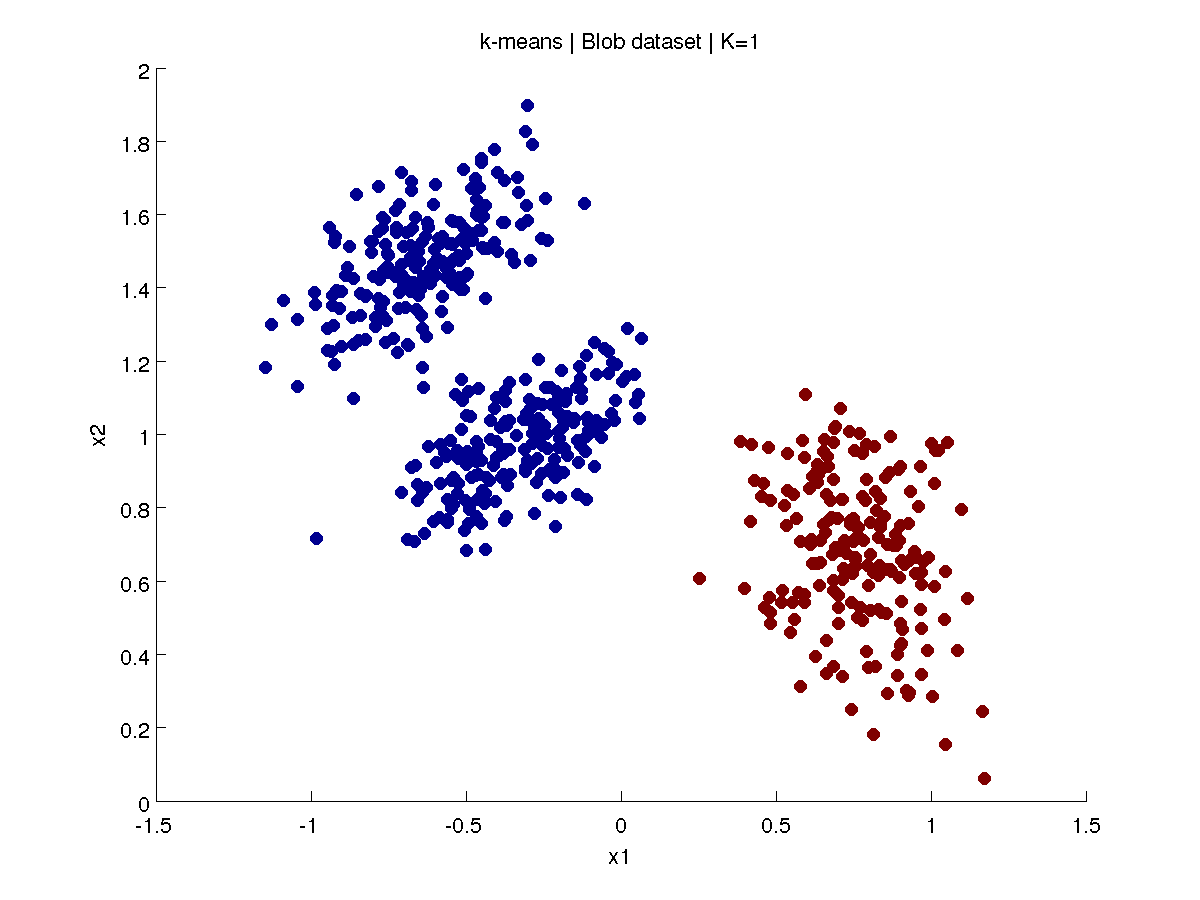
\includegraphics[width=\linewidth]{blob-2}	
			\caption{Problem 4.2 Blob Dataset $k=2$}
	\end{minipage}
	\begin{minipage}{0.5\linewidth}
		%\begin{figure}
			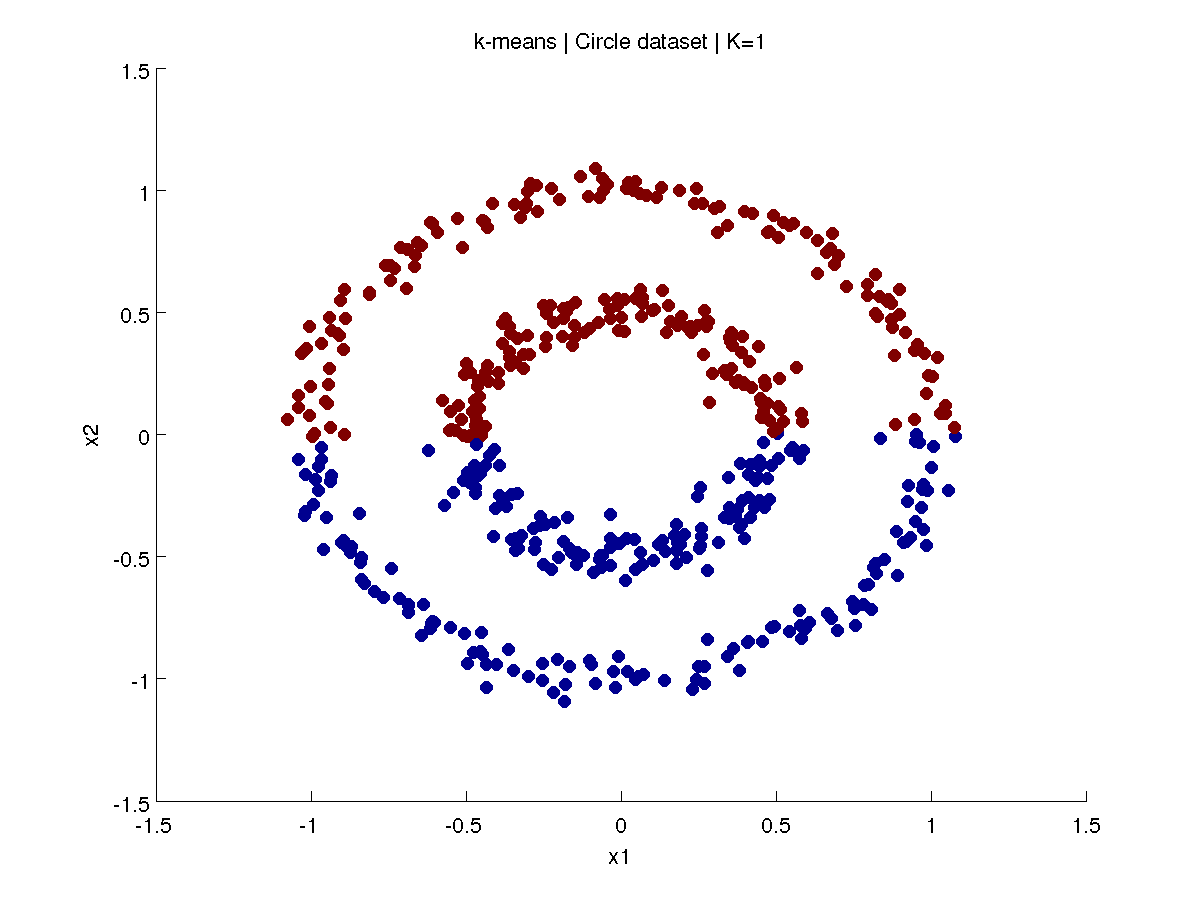
\includegraphics[width=\linewidth]{circle-2}
			\caption{Problem 4.2 Circle Dataset $k=2$}
		%\end{figure}
	\end{minipage}	
	\begin{minipage}{0.5\linewidth}
		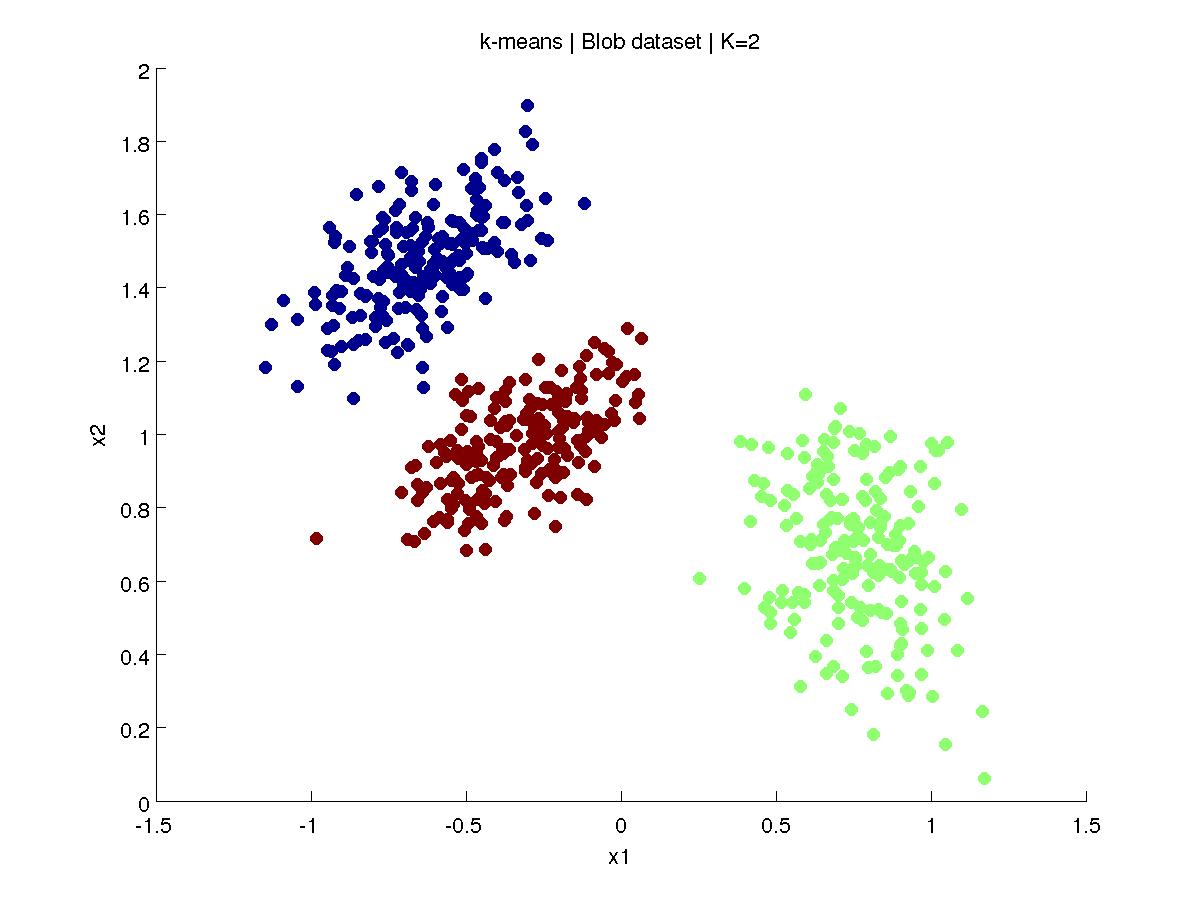
\includegraphics[width=\linewidth]{blob-3}	
		\caption{Problem 4.2 Blob Dataset $k=3$}
	\end{minipage}
	\begin{minipage}{0.5\linewidth}
		%\begin{figure}
		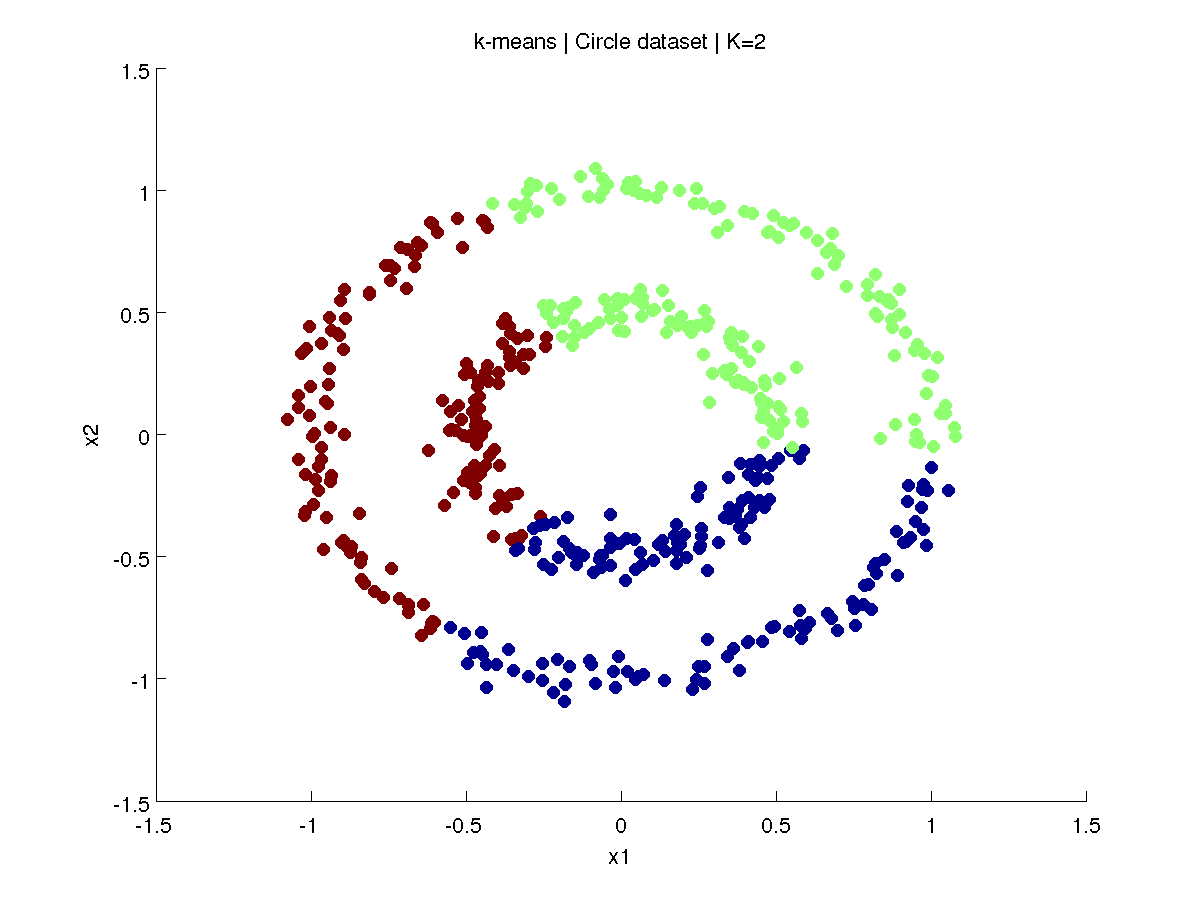
\includegraphics[width=\linewidth]{circle-3}
		\caption{Problem 4.2 Circle Dataset $k=3$}
		%\end{figure}
	\end{minipage}	
		\begin{minipage}{0.5\linewidth}
			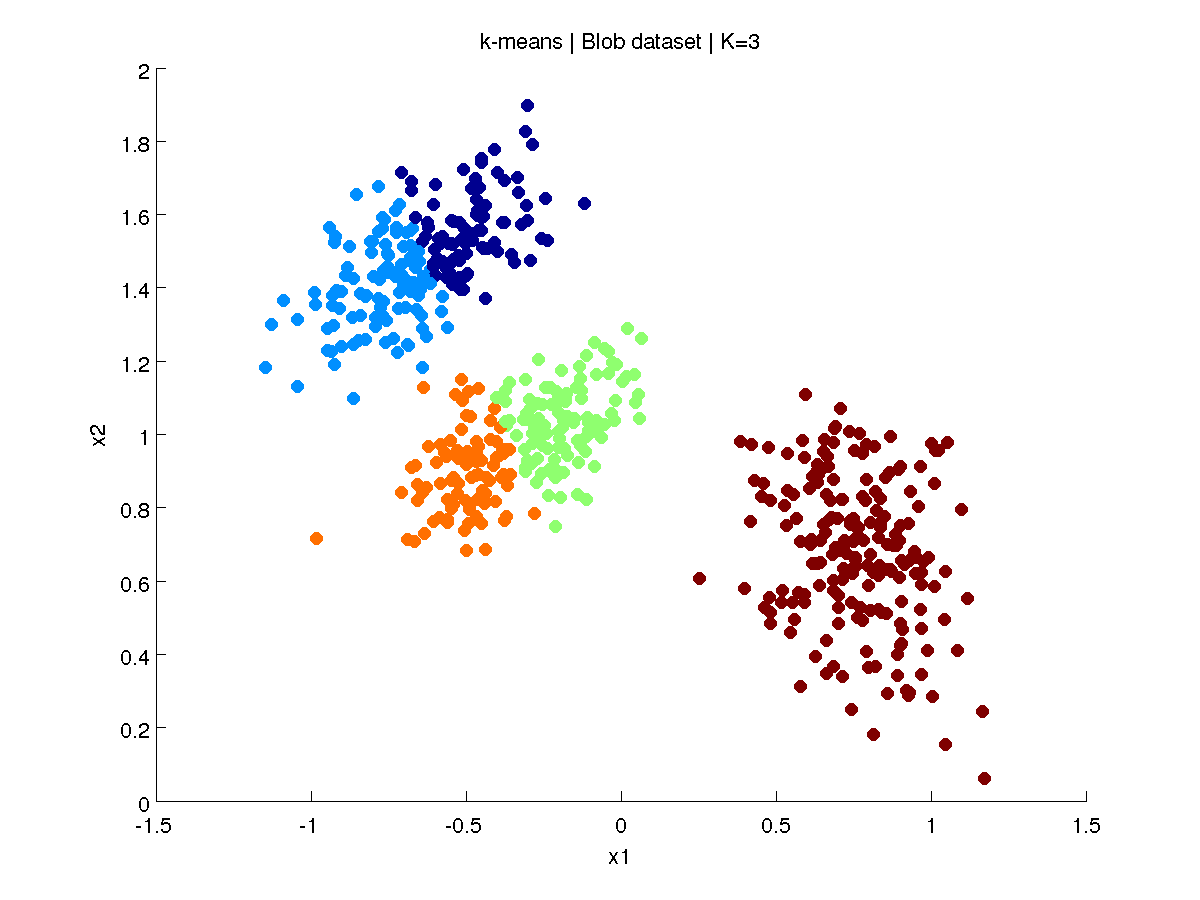
\includegraphics[width=\linewidth]{blob-5}	
			\caption{Problem 4.2 Blob Dataset $k=5$}
		\end{minipage}
		\begin{minipage}{0.5\linewidth}
			%\begin{figure}
			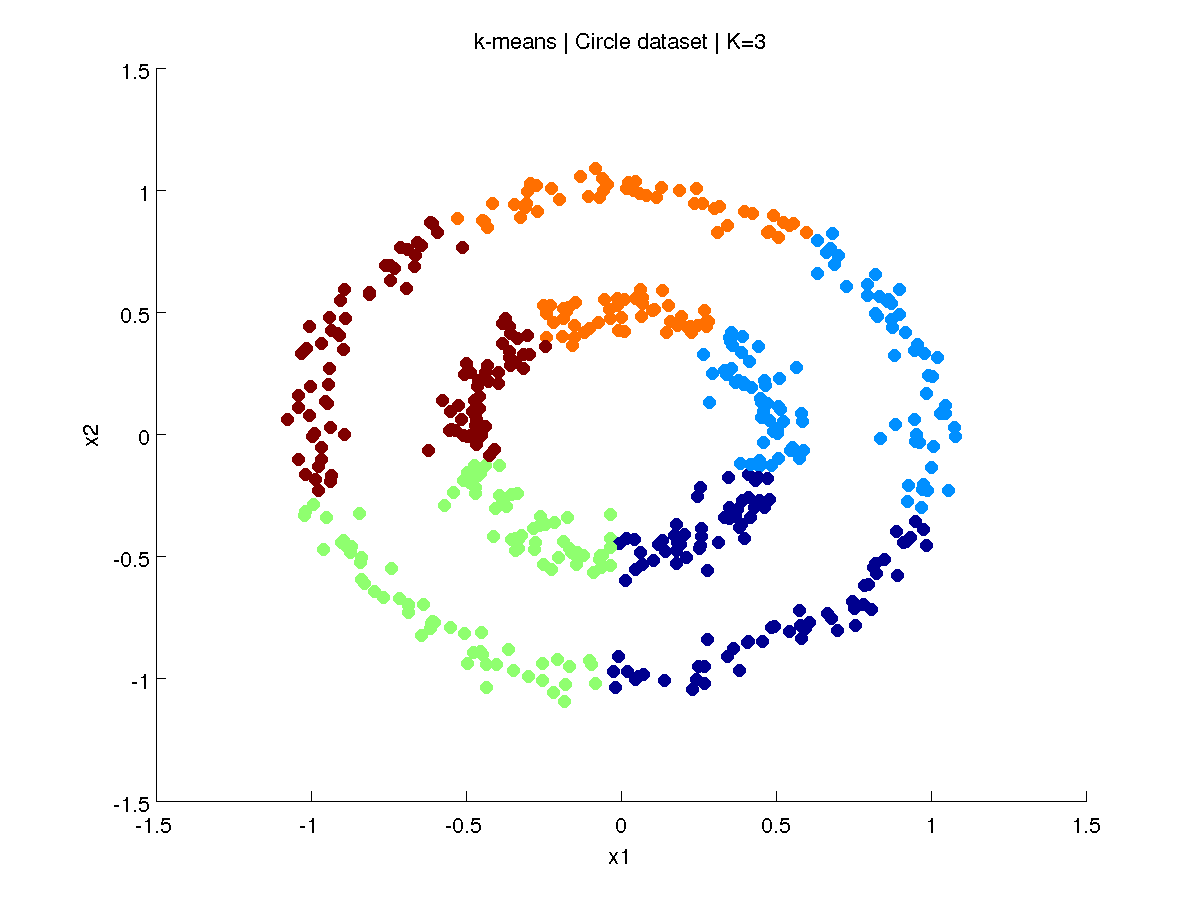
\includegraphics[width=\linewidth]{circle-5}
			\caption{Problem 4.2 Circle Dataset $k=5$}
			%\end{figure}
		\end{minipage}	
		\end{figure}
	%\problemAnswer{

	%	}
\end{homeworkSection}
\newpage

\begin{homeworkSection}{Problem 4.3(a)}
	\problemAnswer{
		Choice of Kernel = RBF: 
		$$
		K(x,x') = \exp(-\frac{||x-x'||^2}{2\sigma^2})
		$$
		with $\sigma = 0.1$
		
		}
\end{homeworkSection}	
	\begin{homeworkSection}{Problem 4.3(b)}
		\begin{figure}
			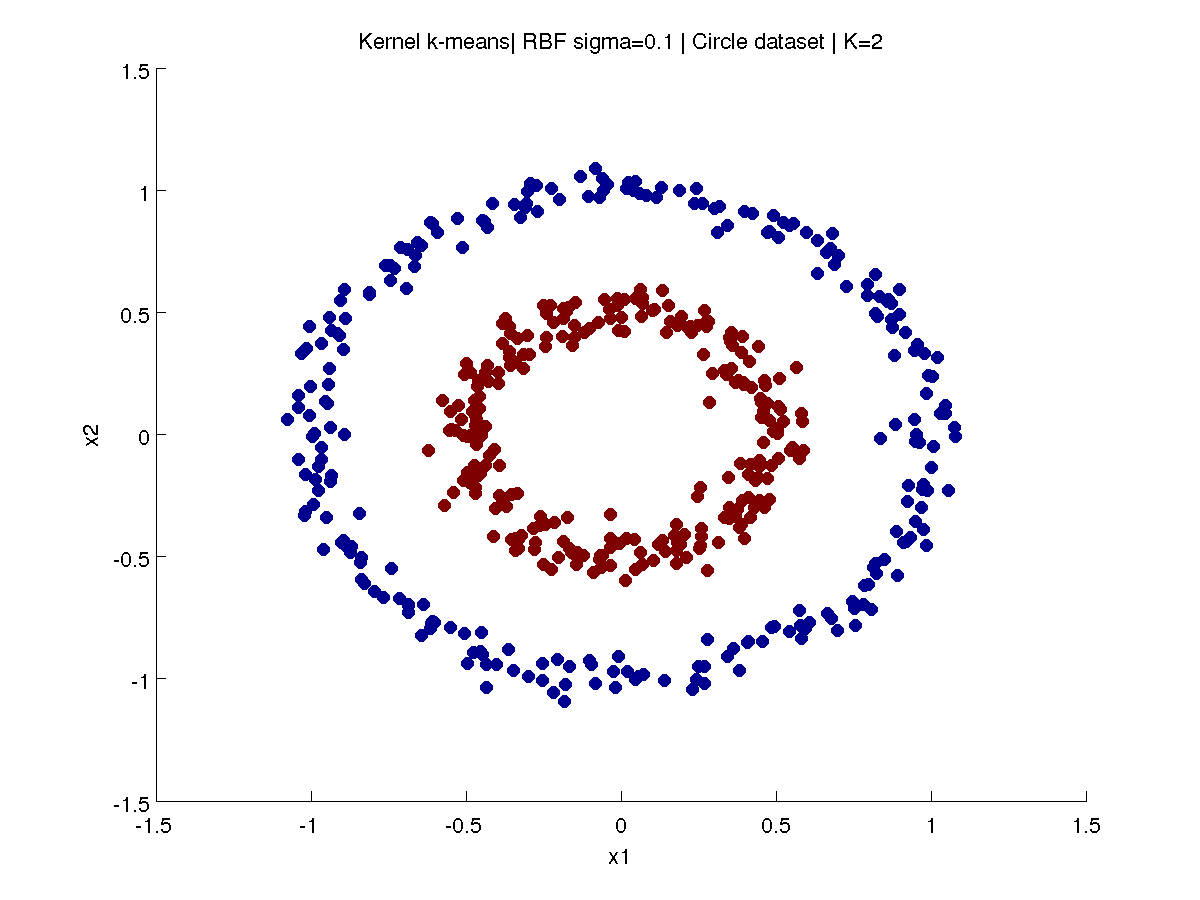
\includegraphics[width=\linewidth]{kcircle-2}
			\caption{Problem 4.3(b) Kernel k-means with RBF kernel creates separate clusters}
		\end{figure}
\end{homeworkSection}



\begin{homeworkSection}{Problem 4.4(a)}
\begin{figure}
	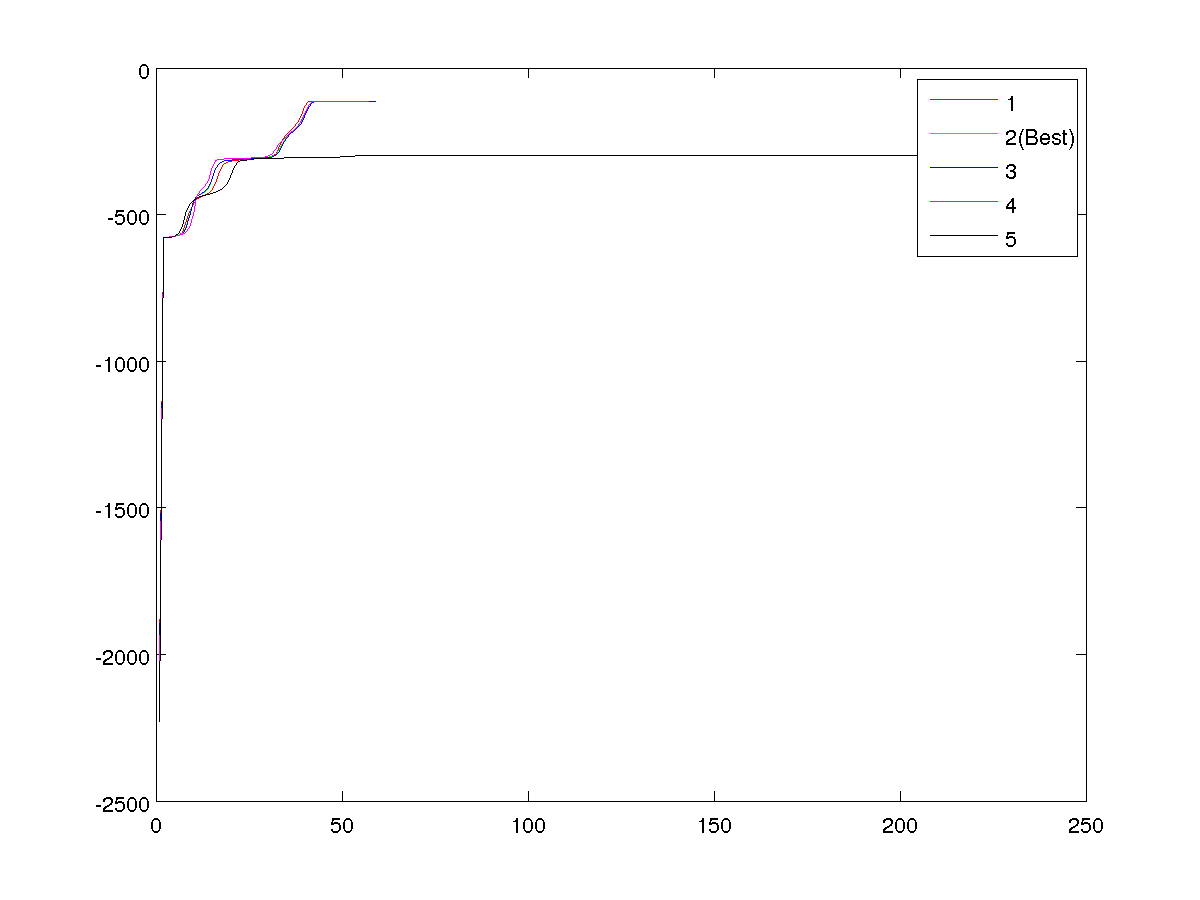
\includegraphics[width=\linewidth]{ll}
	\caption{Problem 4.4(a) Log likelihood versus iteration for GMM with 3 mixtures and 5 different initializations}
\end{figure}

\end{homeworkSection}

\begin{homeworkSection}{Problem 4.4(b)}
	\begin{figure}
		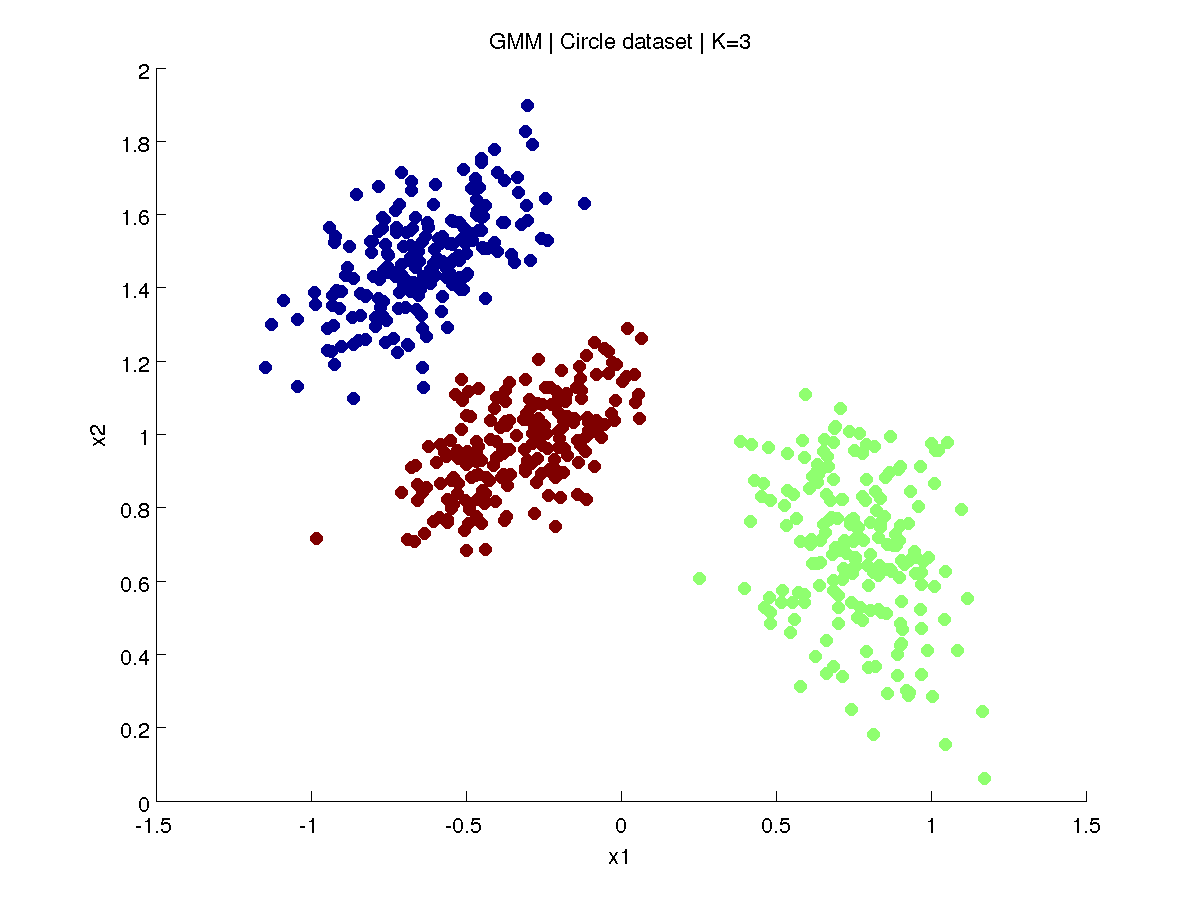
\includegraphics[width=\linewidth]{ll-scatter}
		\caption{Problem 4.4(b) GMM showing most likely assignments}
	\end{figure}
	\newpage
	\problemAnswer{
		$\mu_i$: Centroid of  cluster $i$\\
		$\sigma_i$: Covariance of cluster $i$
		
	   \begin{eqnarray*}
		 \mu_1  = (-0.6395,1.4746)\\
		 \sigma_1 = \begin{pmatrix}
		 	0.0360 &   0.0155\\
		 	0.0155 &   0.0194
		 \end{pmatrix}
   \end{eqnarray*}
   	   \begin{eqnarray*}
		 \mu_2 = (0.7590,0.6798)\\
		 \sigma_2 = \begin{pmatrix}
		 	  0.0272  & -0.0084\\
		 	  -0.0084  &  0.0404		 	  
		 \end{pmatrix}\\
		    \end{eqnarray*}
		    \begin{eqnarray*}
		 \mu_3 = ( -0.3259,0.9713)\\
		 \sigma_3 = \begin{pmatrix}
		 	 0.0360  &  0.0146\\
		 	 0.0146  &  0.0163
		 \end{pmatrix}
	   \end{eqnarray*}
	   }
	   
	   
\end{homeworkSection}
\end{homeworkProblem}
\end{document}
